\documentclass[table]{beamer}
\usetheme{Madrid}  % https://hartwork.org/beamer-theme-matrix/
% \usecolortheme{beaver}
\setbeamertemplate{enumerate item}[default]
\setbeamertemplate{enumerate subitem}[default]

\usepackage{graphicx}
\usepackage{xcolor}
\usepackage{subcaption}
\usepackage{tikz}

\newcommand*\struttert[1]{\vrule width0pt height0pt depth#1\relax}
\newcommand{\round}[1]{\left \lfloor #1 \right \rceil}
\newcommand{\notee}[2]{#1${}_{#2}$}


\begin{document}
\title[Real-time monophonic pitch estimation]{{\LARGE Real-time monophonic pitch estimation for guitar driven sound synthesis}}
\author[Luc de Jonckheere]{\textbf{{\large Luc de Jonckheere}}~\\~\\{\small Supervised by:\\Erwin Bakker\\Michael Lew}}
\date[29 Augustus 2022]{29 Augustus 2022}
\institute[]{{\normalsize LIACS\\~Leiden University}}
\logo{
\includegraphics[width=0.225\textwidth]{figures/logoleiden}}

% Welcome everybody...
\frame{\titlepage}


% \begin{frame}
% \frametitle{Contents}
%     \begin{itemize}
%         \item Motivation and goals
%         \item Preliminary knowledge
%         \item Basic estimator
%         \item HighRes estimator
%         \item Conclusions
%         \item Digistring demo
%     \end{itemize}
% \end{frame}


% So what is real-time monophonic pitch estimation? Pitch estimation is detecting what note is played in a signal. Real-time refers to the fact that we want to estimate the note while the musician is playing it, such that it can be used for sound synthesis. We set a limit of 20 milliseconds on the pitch estimation latency. Exceeding this real-time constraint causes our synthesizer to fail as a live instrument. Lastly, we focus on monophonic pitch estimation. Here, we assume the signal contains at most one note at a time. It is much easier to perform monophonic pitch estimation compared to polyphonic pitch estimation. Using special hexaphonic pick-ups, which records each string individually, we can view a guitar as a six-way monophonic instrument.
% What motivated me to study this is because I always wanted to be able to control synthesizers using my guitar instead of something like a keyboard. There are no open-source real-time pitch estimation programs available, so I decided to make one.
% This leads to the main goal of my thesis, which is creating a real-time pitch estimation algorithm. Furthermore, I want to synthesize sounds based on my estimations and drive existing synthesizers.
\begin{frame}
\frametitle{Introduction}
% \frametitle{Motivation and goals}
    {\large \textbf{Real-time monophonic pitch estimation}}
    \begin{itemize}
        \item Pitch estimation: Measure pitch of signal/played note
        \item Real-time: While the musician is playing it
        \begin{itemize}
            \item[{\LARGE \rotatebox[origin=c]{180}{$\Lsh$}}] Real-time constraint: 20 ms
        \end{itemize}
        \item Monophonic: One note at the time
    \end{itemize}
    \vfill

    {\large \textbf{Motivations}}
    \begin{itemize}
        \item Drive synthesizer with a guitar
        \item No open source real-time pitch estimation applications available
    \end{itemize}
    \vfill

    {\large \textbf{Goals}}
    \begin{enumerate}
        \item Create a real-time pitch estimation algorithm
        \item Synthesize audio based on estimation
    \end{enumerate}
    % \bigskip

    % Goal 2-3 $\rightarrow$ clear division of front-end and back-end
\end{frame}
% Before we can get into pitch estimation, some preliminary knowledge is required


% First, let me explain how audio works in computers. An sound wave, visuallized by the red line, is encoded as a series of equally spaced samples, visuallized by the blue dots with gray lines. Each sample represents the height of the audio waveform at a specific point in time. The audio format determines how each sample is encoded. The sample rate determines how many samples per second are used to describe the sound wave.
\begin{frame}
\frametitle{Preliminary knowledge}
    {\large \textbf{Audio in computers}}
    \begin{itemize}
        \item Audio format
        \item Sample rate ($f_{\text{SR}}$)
    \end{itemize}

    \begin{figure}[H]\vspace{-14mm}
        \begin{subfigure}{.45\textwidth}
            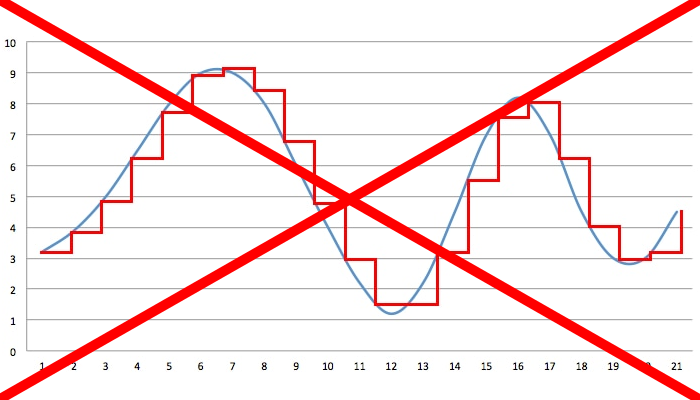
\includegraphics[width=\linewidth]{figures/no_sampling.png}
        \end{subfigure}
        \begin{subfigure}{.54\textwidth}
            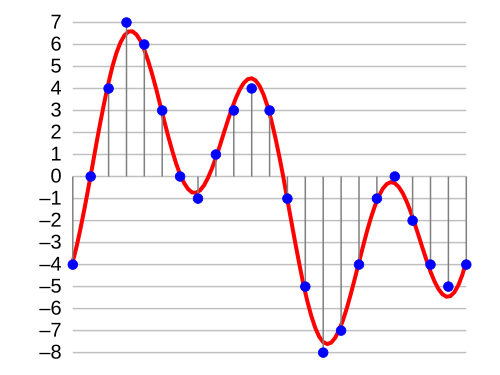
\includegraphics[width=\linewidth]{figures/sampling.png}
        \end{subfigure}
    \end{figure}
\end{frame}


% Central to our pitch estimation method is the Fourier transform. The Fourier transform transforms a function of time to a complex valued function of frequency. To visualize this, take a look at this picture. On the left, we see a sound wave. We can describe the sound wave as a sum of sine waves. The Fourier transform gives us a function which describes the signal through sine waves. The Fourier transform works on continuous functions and assumes an infinite time interval. Concepts such as continuous and infinite cannot be represented by a computer and, consequently, the discrete Fourier transform has to be used for Fourier analyses on computers.
\logo{}
\begin{frame}
\frametitle{Preliminary knowledge}
    {\large \textbf{Fourier transform}}
    \begin{figure}[H]
        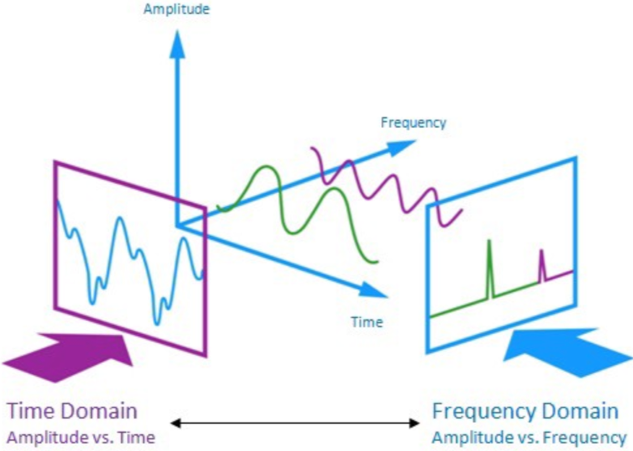
\includegraphics[width=0.75\linewidth]{figures/fourier3.png}
    \end{figure}
\end{frame}
\logo{
\includegraphics[width=0.225\textwidth]{figures/logoleiden}}


% The DFT works on a sequence of equally spaced samples, which we call a frame, and transforms it in an equal number of bins. The frequency resolution of a DFT is determined by dividing the sample rate by the number of samples in a frame. This implies that if we acquire more samples, we get a higher resolution frequency domain at the cost of a higher latency. We can only detect frequencies up to half the sample rate. Each bin is represented by a complex number and corresponds to one specific frequency. From this complex number we can compute the amplitude and phase offset of that specific frequency component. All frequencies in the signal which do not exactly fit in a bin are spread out over the other bins. This effect is called spectral leakage.
\begin{frame}
\frametitle{Preliminary knowledge}
    {\large \textbf{Fourier transform}}
    \begin{itemize}
        \item Function of time $\rightarrow$ function of frequency
        \item Continuous/infinite $\not \in$ computers \ $\rightarrow$ \ DFT
    \end{itemize}
    \bigskip

    {\large \textbf{Discrete Fourier transform} (DFT)}
    \begin{itemize}
        \item Frame of samples $\rightarrow$ frequency bins
        \item Fourier resolution = sample rate / frame size = frame time ${\!}^{-1}$
        \item Nyquist frequency = sample rate / 2
        \item Each bin corresponds to one frequency
        \item Spectral leakage
    \end{itemize}
\end{frame}


% Here, we can see an example of spectral leakage. In the top image we can see the signal exactly matches a bin and no leakage occurs. However, at the bottom image, the signal is exactly between two bins and we measure many frequencies.
\begin{frame}
\frametitle{Preliminary knowledge}
    \begin{figure}[H]\vspace{+5mm}
        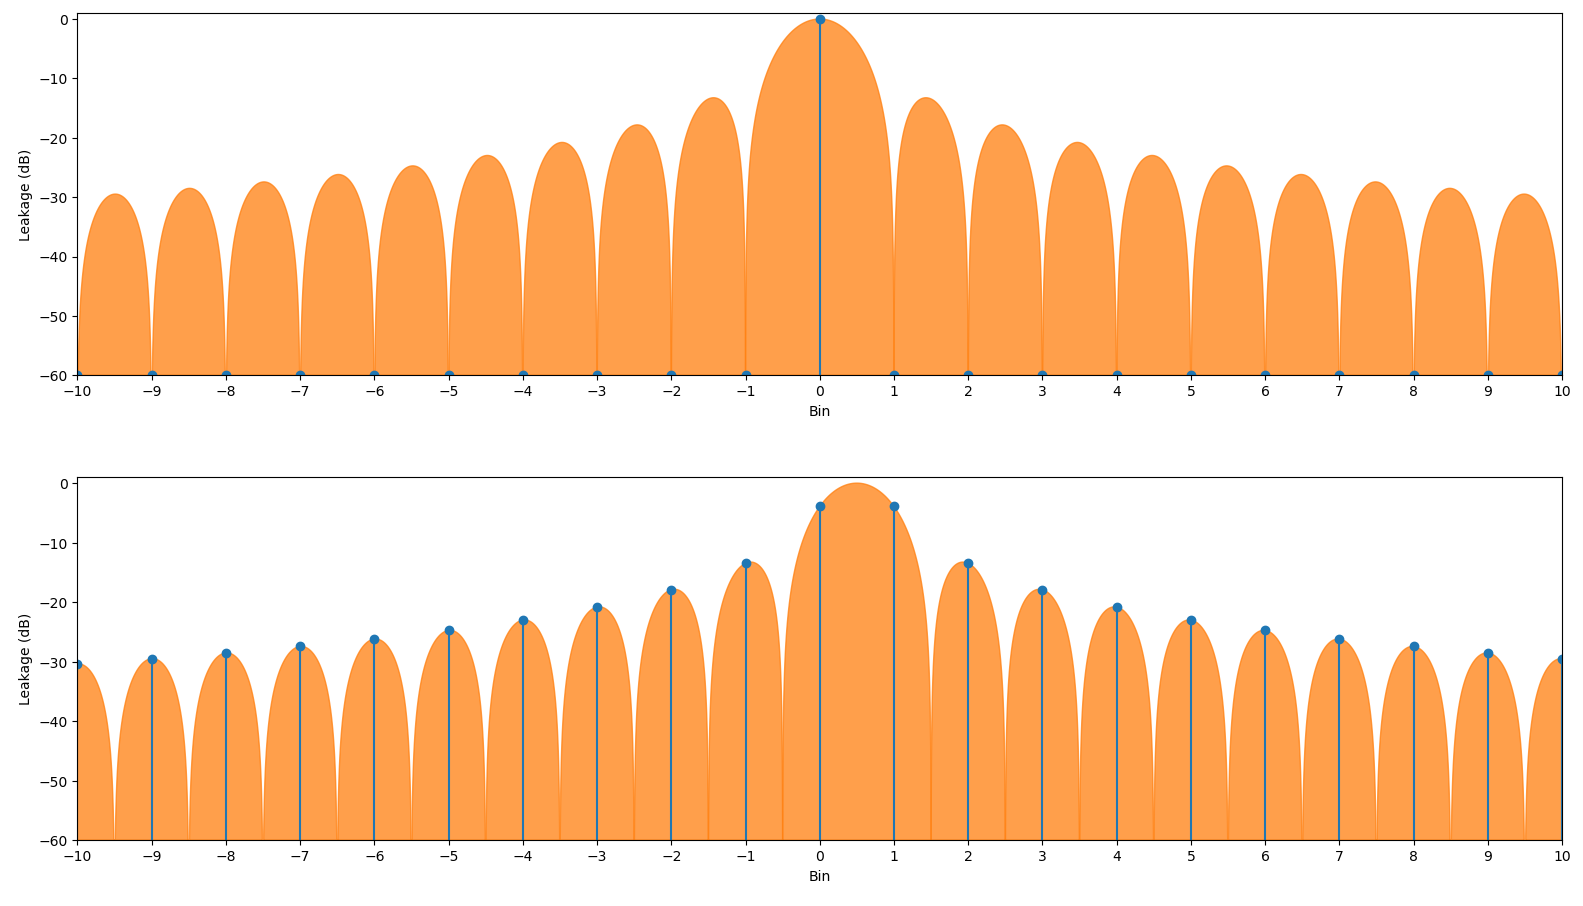
\includegraphics[width=\linewidth]{figures/winleak.png}
    \end{figure}
\end{frame}


% Leakage occurs due to the fact that the DFT regards the signal as infinitely repeating. This may cause distortions around the frame borders. If we for example take the signal between the red lines, we can see the distortion in the second image.
% We can control spectral leakage using window functions. They smooth the distortions around the frame borders. Different window functions have different leakage behavior, as can be seen on the right.
\begin{frame}
\frametitle{Preliminary knowledge}
    \begin{figure}[H]
        \begin{subfigure}{.40\textwidth}
            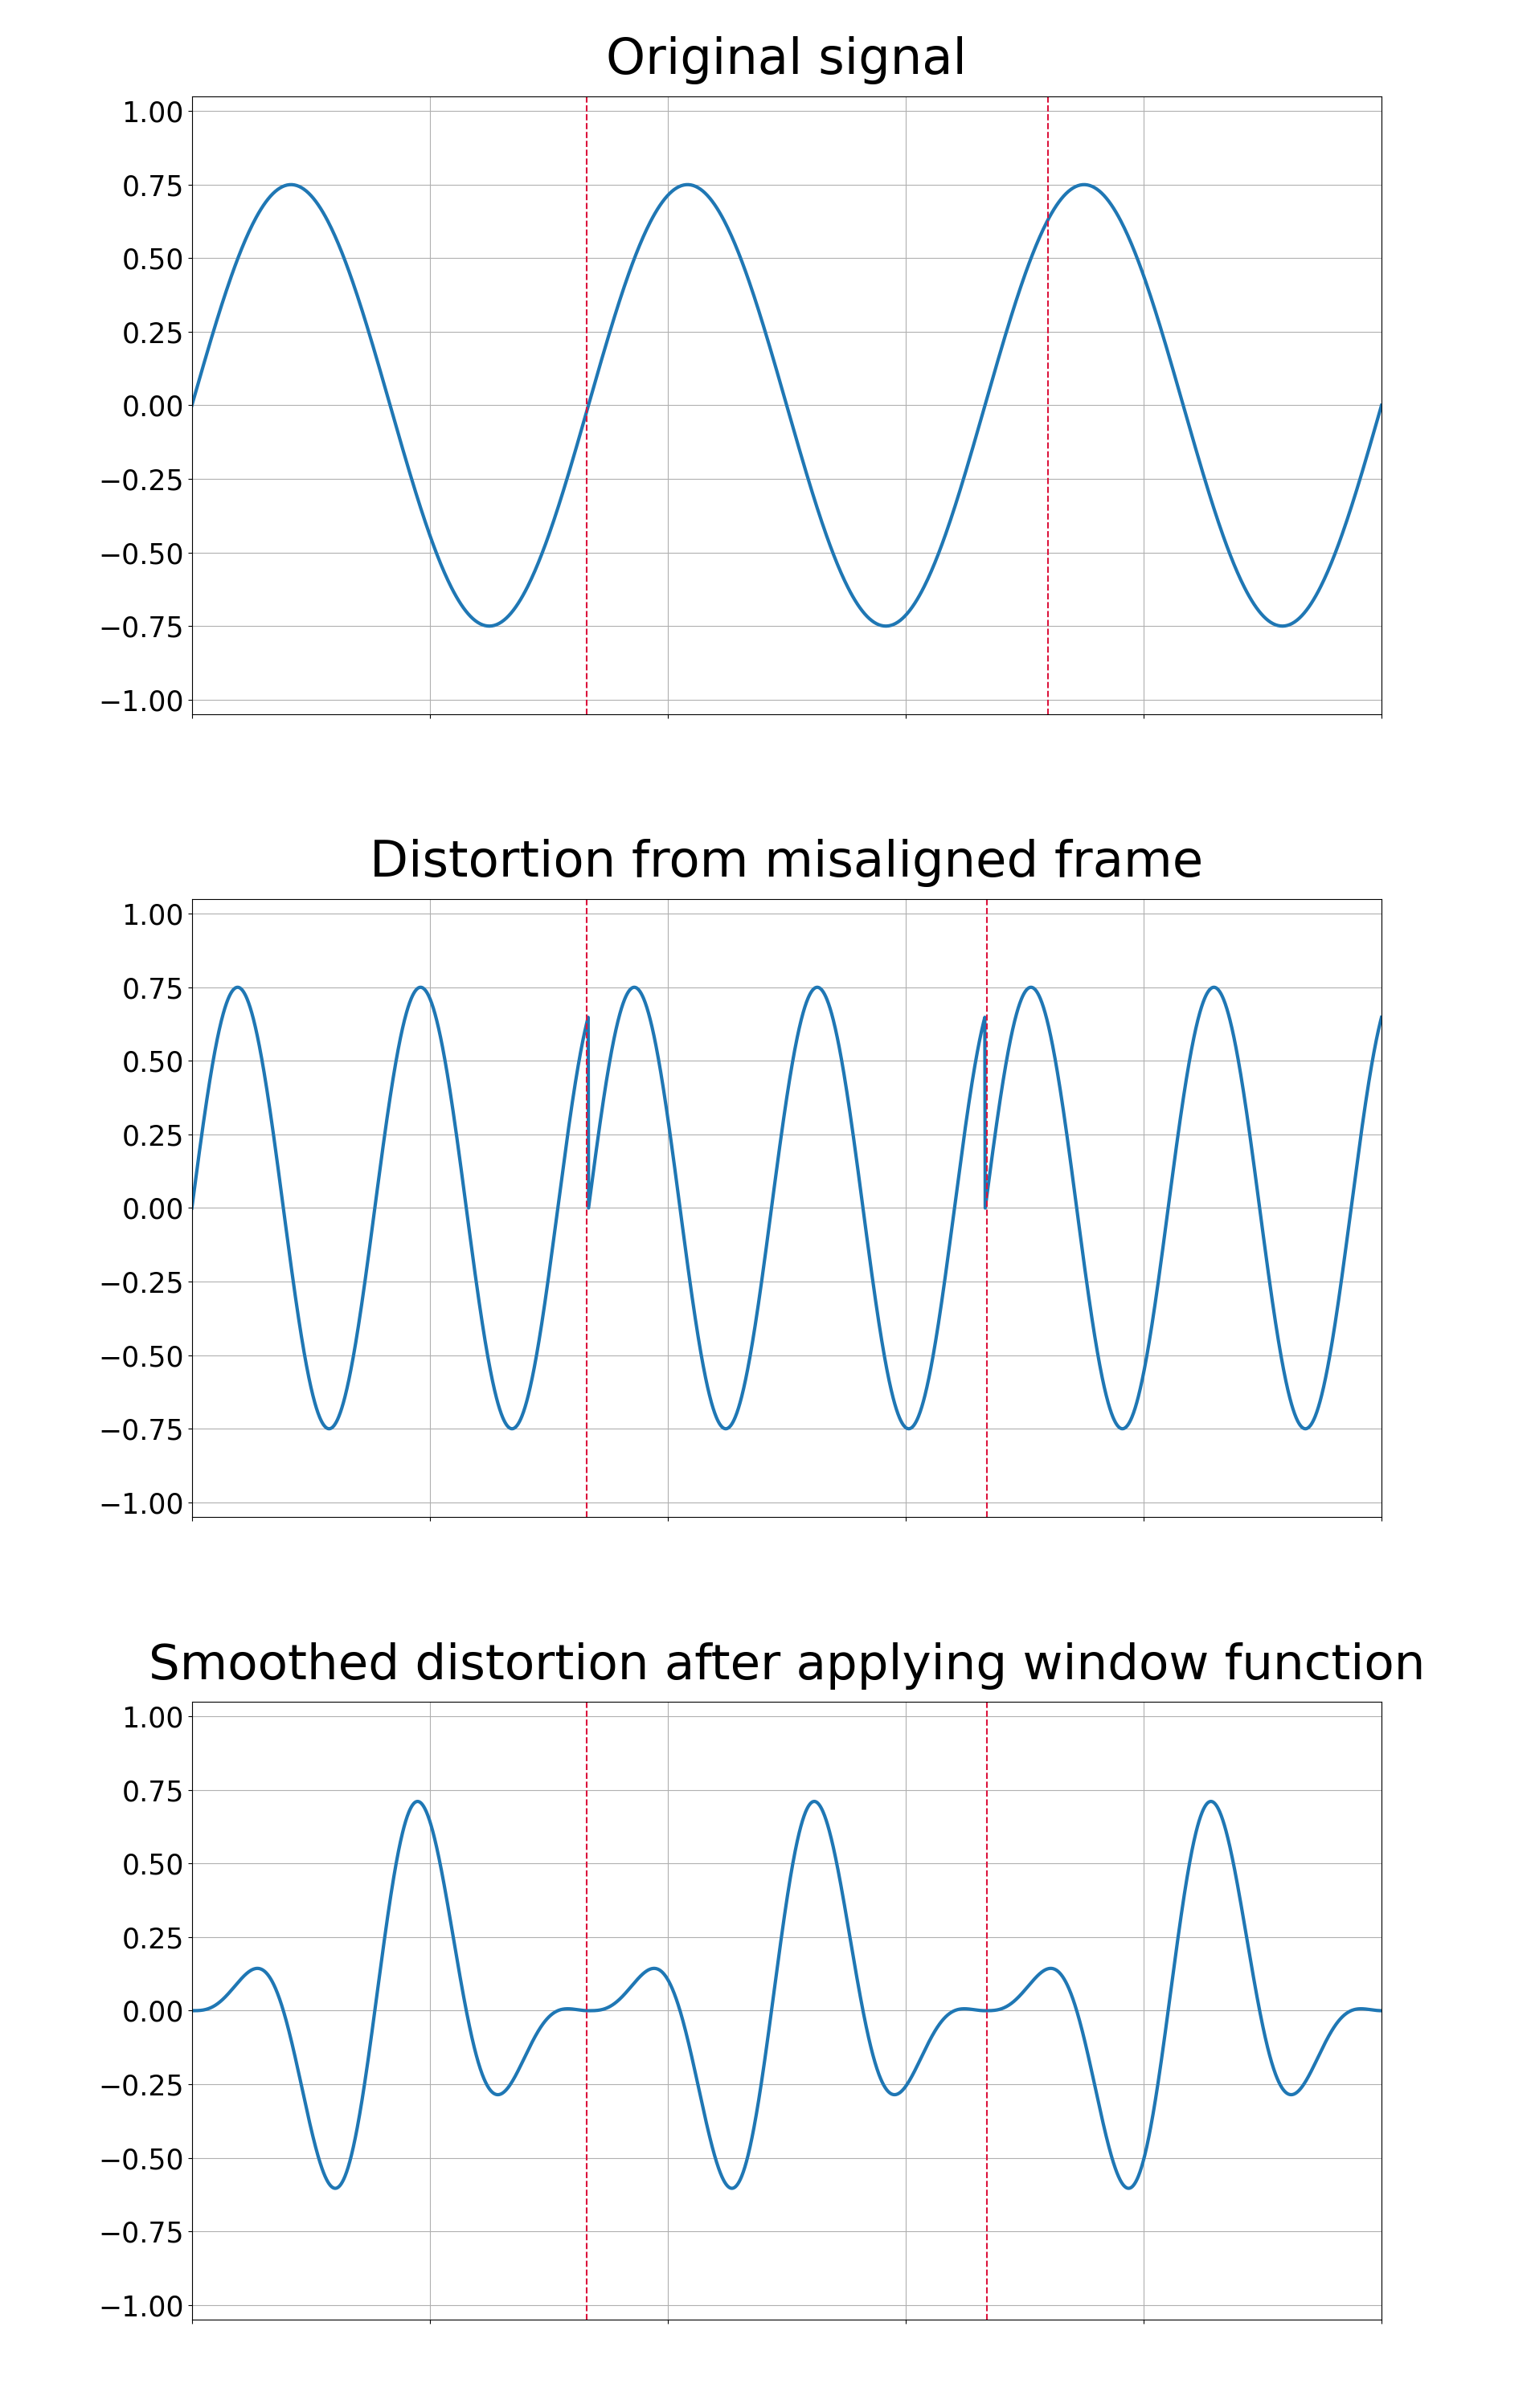
\includegraphics[width=\linewidth]{figures/framedistortion.png}
        \end{subfigure}
        \hspace{+4.7mm}
        \begin{subfigure}{.54\textwidth}
            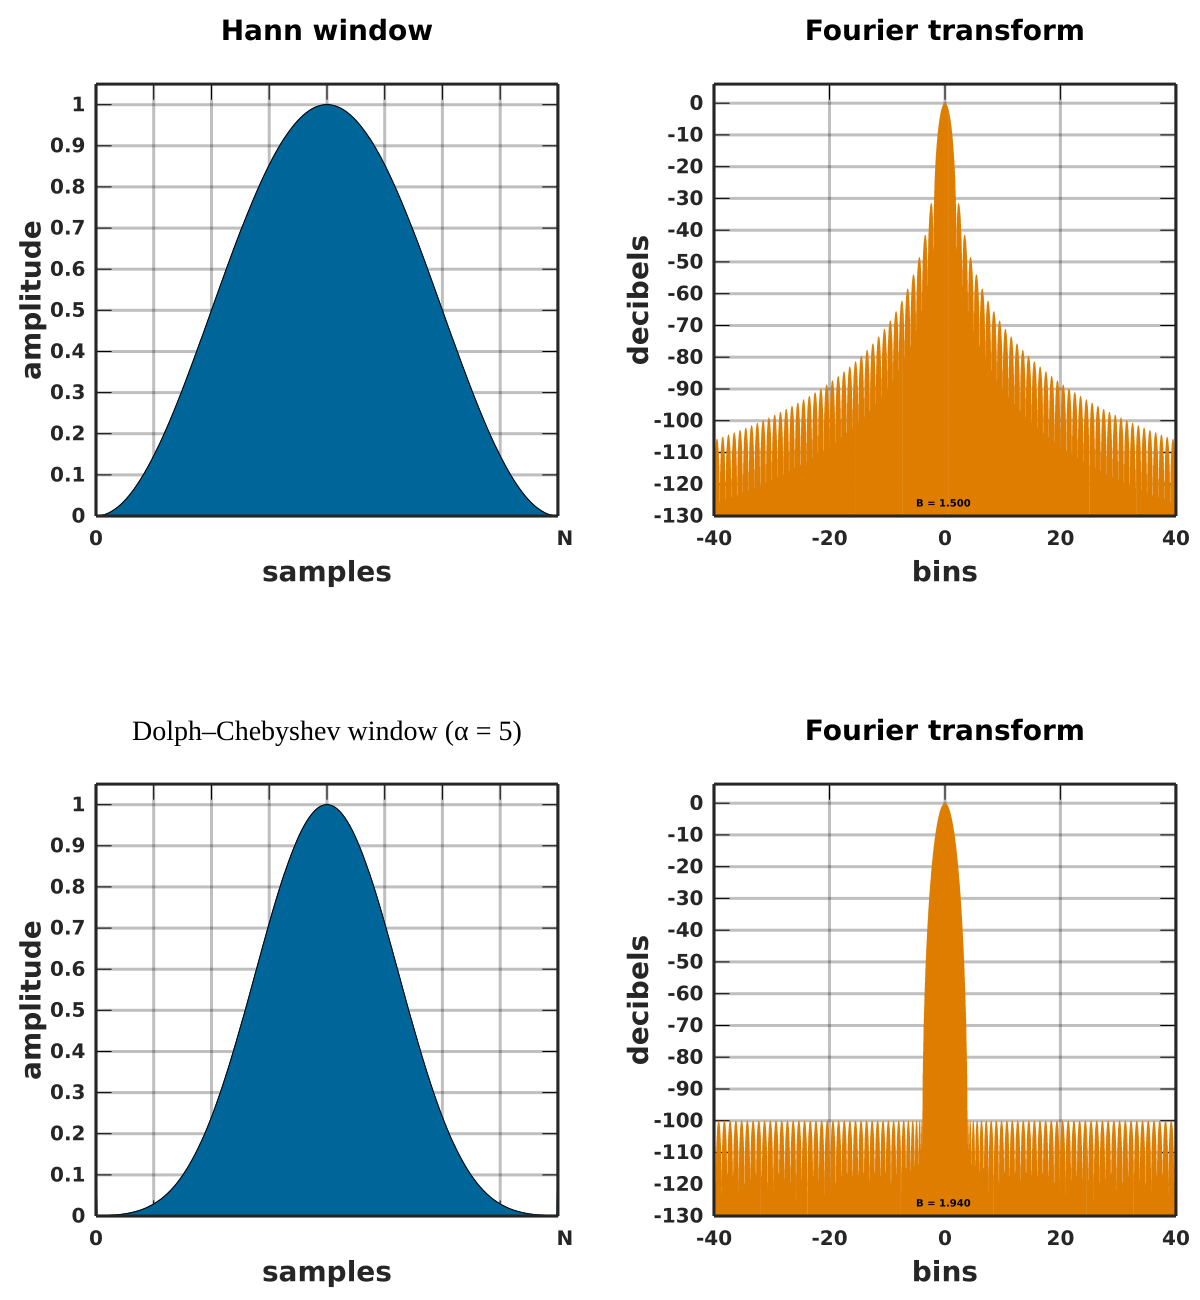
\includegraphics[width=\linewidth]{figures/windows.png}
        \end{subfigure}
    \end{figure}
\end{frame}


% In order to interpret the results of the Fourier transform, we need to understand some music theory and understand how sound is generated from a guitar.
% Most modern music uses the 12 tone equal temperament music system, which describes the relation between notes. Then, by choosing a tuning note, we can calculate the frequencies associated with each note. Instead of using the tradition note names A to G, we use MIDI note numbers, as it allows us to describe every note using integers.
% When playing notes on instruments, many frequencies are generated. Most notable are the fundamental frequency and its overtones. The fundamental frequency is the main frequency we associate with a note. Integer multiples of the fundamental frequency can resonate and give rise to harmonic overtones. Many other frequencies are generated along with the fundamental and its overtones. The instrument specific pattern of these frequencies is called the timbre of the instrument. These frequencies are of low amplitude and we can simply ignore them. When strumming a note, a percussive sound is generated. This is called a transient. Percussive sounds behave very chaotically and we consider them noise.
\begin{frame}
\frametitle{Preliminary knowledge}
    {\large \textbf{Music theory}}
    \begin{itemize}
        \item 12 tone equal temperament (12-TET)
        \item Tuning note (\notee{A}{4} = 440 Hz)
        \item MIDI note numbers (\notee{A}{4} = 69)
    \end{itemize}
    \bigskip

    {\large \textbf{Physics of sound}}
    \begin{itemize}
        \item Fundamental and overtones
        \item Timbre
        \item Transients
    \end{itemize}
\end{frame}


% Using this preliminary knowledge, we can construct a basic pitch estimation algorithm...
\begin{frame}
\frametitle{Basic estimator}
    {\large \textbf{Basic estimator algorithm}}\\
    Given frame of samples $F$ with sample rate $f_{SR}$
    \begin{enumerate}
        \item Apply window function
        \item Fourier transform
        \item Calculate amplitudes of bins
        \item Find bin index with highest amplitude ($i_{\text{max}}$)
        \item Compute frequency of the bin ($f_b = i_{\text{max}} * \frac{f_{\text{SR}}}{|F|}$)
        \item Compute MIDI note number corresponding to frequency\\
        % $\underbrace{\struttert{0.75mm}\round{12 * {}^{2}\!\log{\frac{f_b}{440}}}}_{\text{diverges!}}$
        \begin{itemize}
            \item[{\LARGE \rotatebox[origin=c]{180}{$\Lsh$}}] $\underbrace{\struttert{0.75mm}\round{12 * {}^{2}\!\log{\frac{f_b}{440}}}}_{\text{Distance from \notee{A}{4}}} + \underbrace{\struttert{0.75mm}69}_{\text{\notee{A}{4} MIDI number}}$
        \end{itemize}
    \end{enumerate}
\end{frame}


% This basic estimator has several shortcomings. It has an incredibly high latency of 200 milliseconds in order to obtain a high enough frequency resolution to discern the two lowest notes on a guitar. As the frame times are so long, the frame rate are consequently low as well. All estimations are quantized to the frame time, which is problemetic when the frame time is so long. Furthermore, the first overtone is often louder than the fundamental frequency, causing the basic pitch estimator to estimate the first overtone, also called the octave. Lastly, the estimator has no notion of silence and will always produce a note estimate, even when no note is played.
\begin{frame}
\frametitle{Basic estimator}
    {\large \textbf{Shortcomings}}
    \begin{itemize}
        \item Latency
        \begin{itemize}
            \item[{\LARGE \rotatebox[origin=c]{180}{$\Lsh$}}] \notee{F}{2} - \notee{E}{2} $\approx$ 5 Hz $\rightarrow$ 200 ms frame time
        \end{itemize}
        \item Frame rate
        \begin{itemize}
            \item[{\LARGE \rotatebox[origin=c]{180}{$\Lsh$}}] Frame time ${\!}^{-1}$ $\rightarrow$ 5 FPS
        \end{itemize}
        \item Estimation quantization
        \item Octave problem
        \item Never silent
        % \begin{itemize}
        %     \item Require minimum peak power
        % \end{itemize}
        % \item Always produces an estimation

%     % \vspace{+10mm}
%     % \begin{center}
%         {\large \textbf{Basic estimator demo}}
%     % \end{center}
    \end{itemize}
\end{frame}


% One way to increase the frame rate would be to decrease the frame time. However, this decreases the Fourier resolution. Instead, we can increase the frame rate without decreasing the frame time through overlapping. This image shows a simple overlapping strategy, where we copy a part of the previous frame and fill the rest with new samples, causing our input buffers to overlap.
\begin{frame}[t]
\frametitle{HighRes estimator}
    {\large \textbf{Low frame rate}}
    \begin{itemize}
        \item Decrease frame time $\rightarrow$ decrease Fourier resolution
        \item Overlap frames
    \end{itemize}

    \tikz[remember picture, overlay] {\node[above, anchor=south, outer sep=3.5mm] at (current page.south) {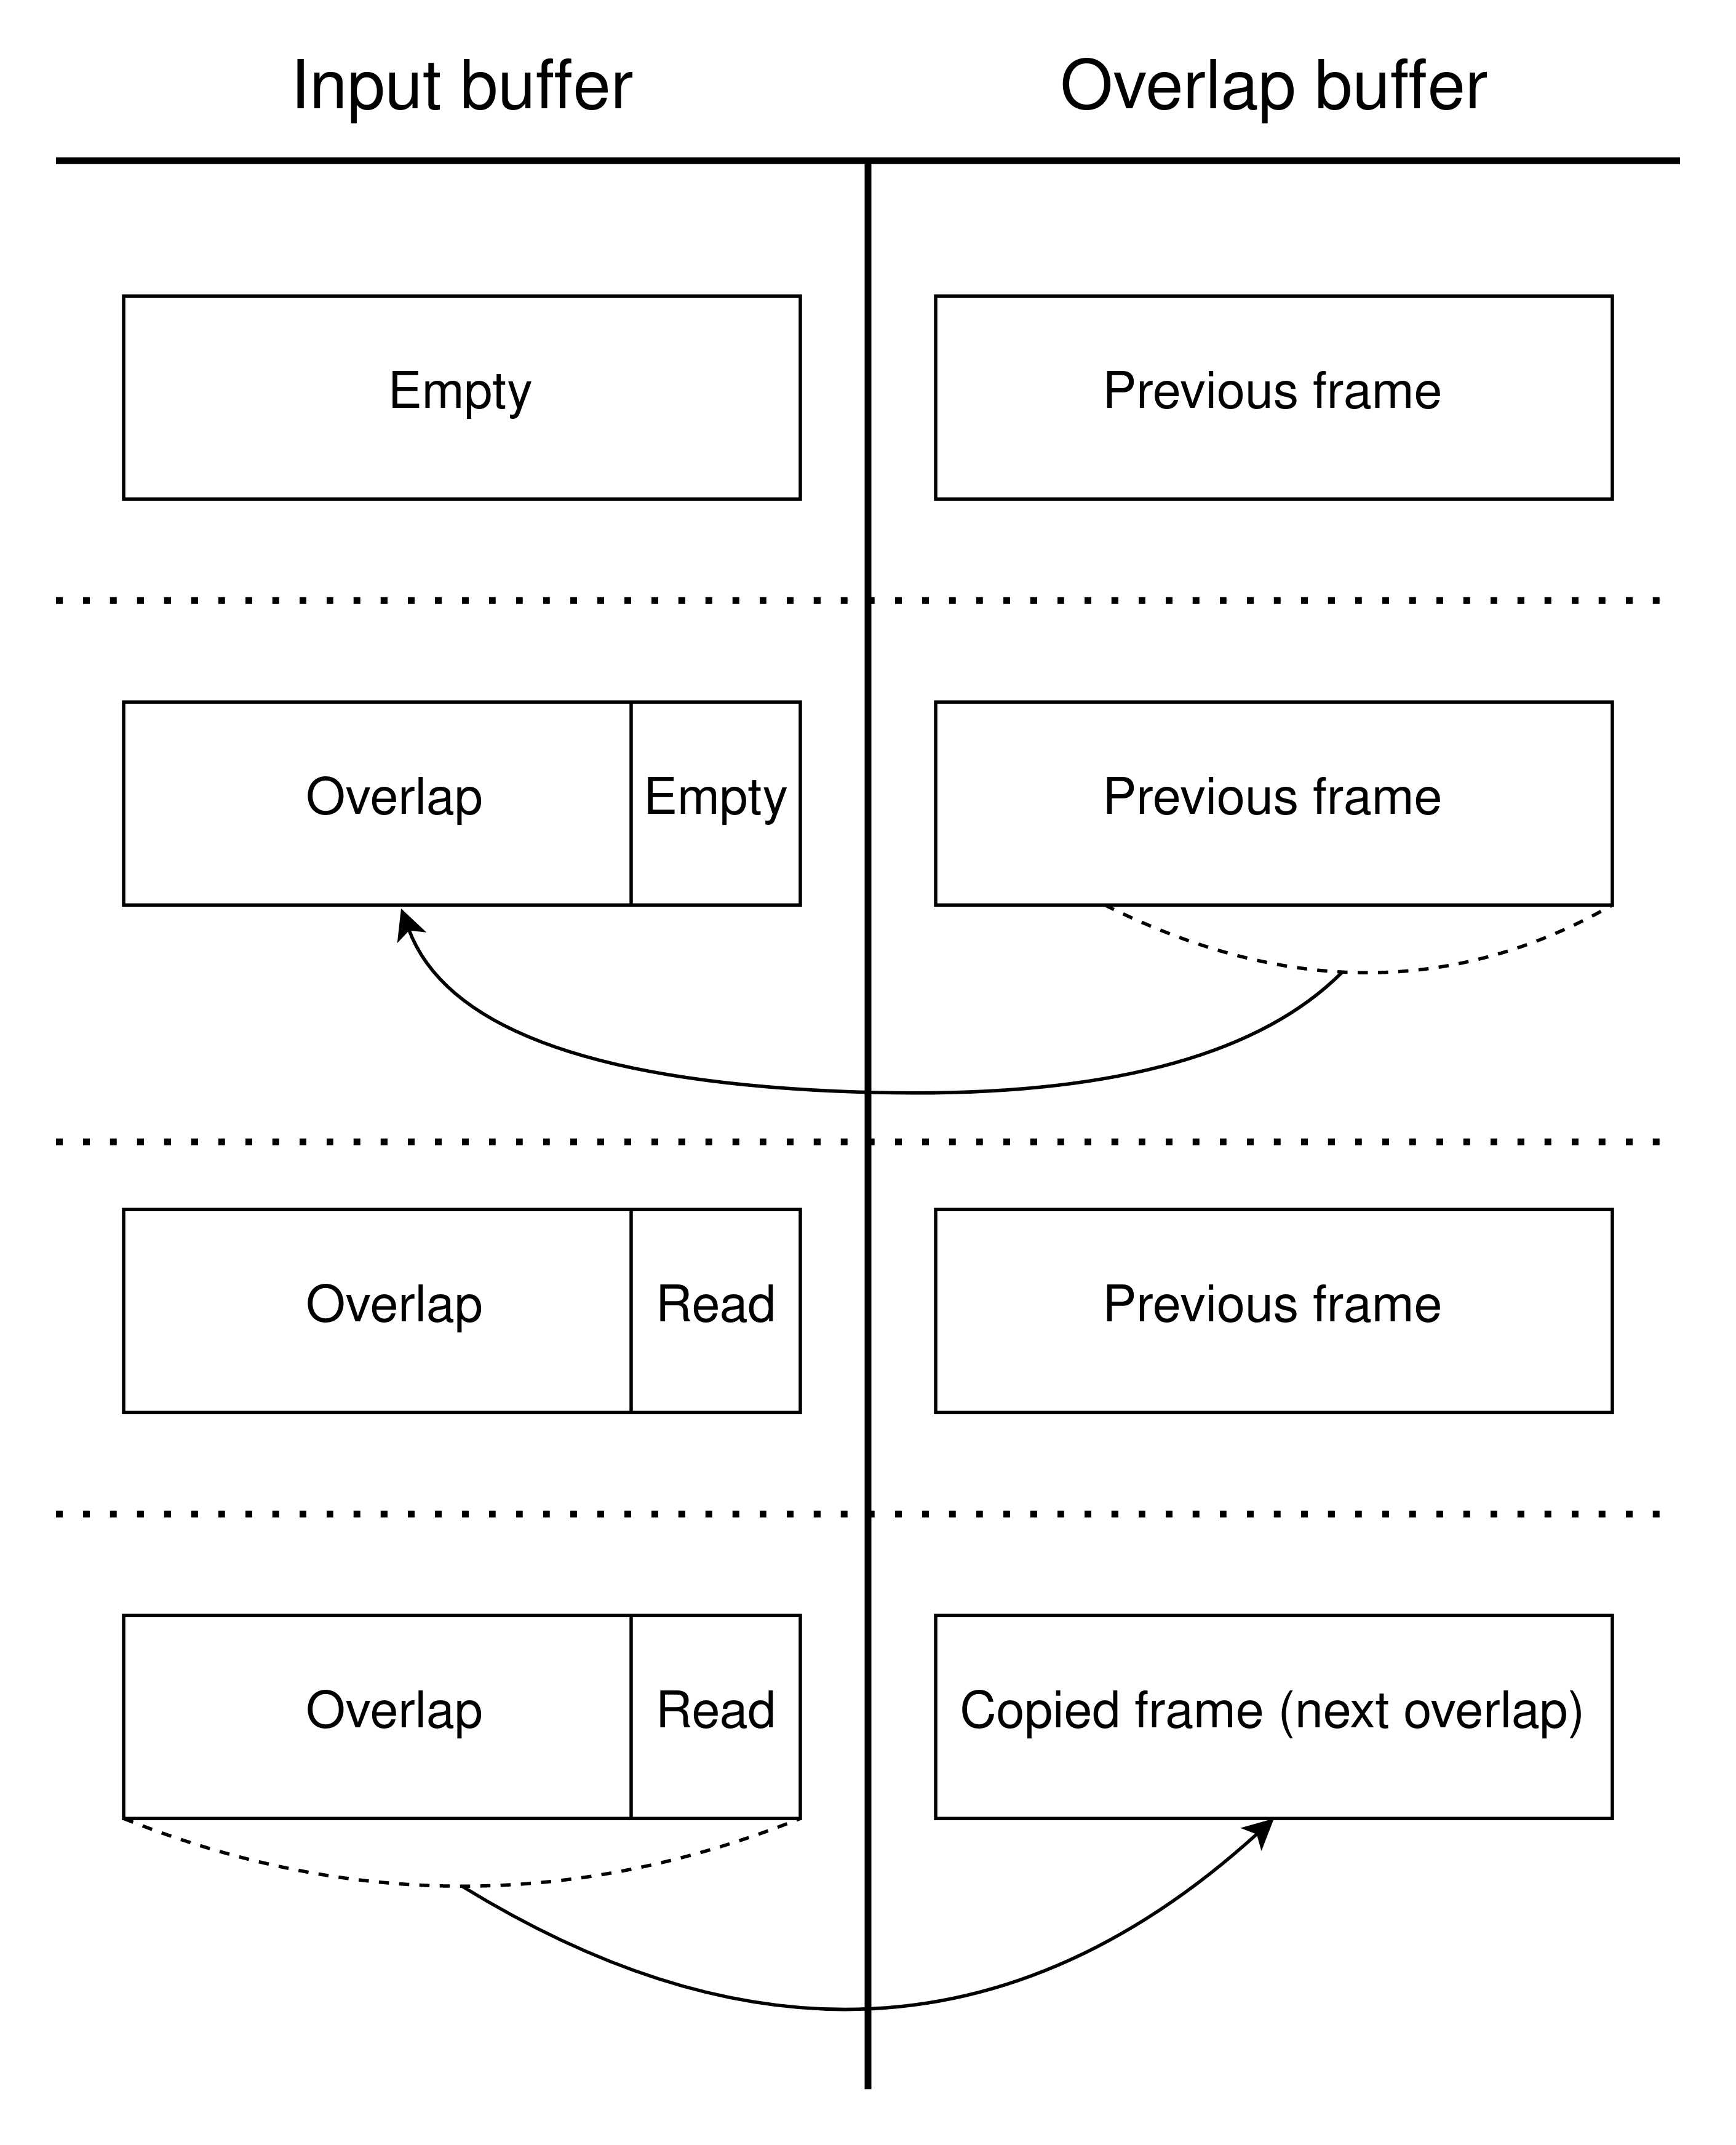
\includegraphics[width=0.42\linewidth]{figures/overlap2.png}};}
\end{frame}


% Our latency is bound by the Fourier resolution. Through clever interpolation, we can remain accurate with less frequency resolution.
% Our first method of interpolation is zero-padding. Here, we simply add zeros to the signal. This increases the frame size and, in turn, it increases the number of output bins. Zero-padding does not add any information, and consequently, two frequencies closer together than the Fourier resolution still form one lobe in the interpolated spectrum. However, as we can see in the figure, the new bins may lie closer to the bin centers, thus interpolating the true peak location.
\logo{}
\begin{frame}
\frametitle{HighRes estimator}
    \vfill
    Low resolution $\rightarrow$ interpolation
    \bigskip

    {\large \textbf{Zero-padding}}
    \begin{itemize}
        \item Increase frame size $\rightarrow$ increase number of bins
        % \item Fourier resolution = sample rate / frame size = frame time ${\!}^{-1}$
        \item No resolution increase, only interpolation!
    \end{itemize}
    \vfill

    \begin{figure}[H]
        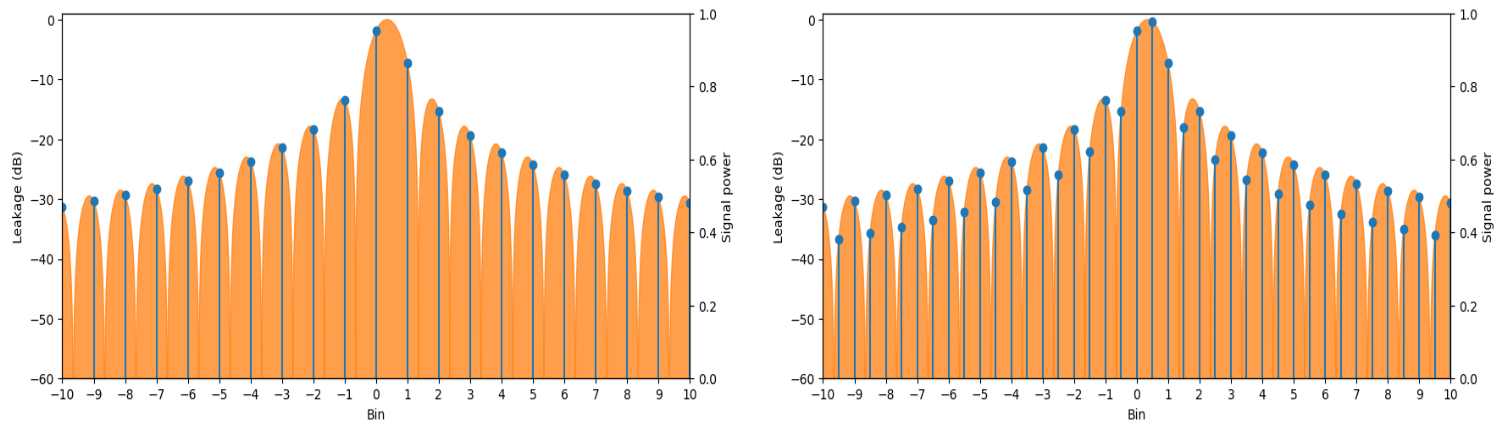
\includegraphics[width=\linewidth]{figures/zeropad.png}
    \end{figure}
\end{frame}
\logo{
\includegraphics[width=0.225\textwidth]{figures/logoleiden}}


% Our second method of interpolation is quadratic interpolation. Here, we fit a Lagrange parabola through the peak bin and its neighbors. The peak of this parapola is the interpolated location. The accuracy of the interpolation increases by scaling the bin height logarithmically. QIFFT works well together with zero-padding.
\logo{}
\begin{frame}
\frametitle{HighRes estimator}
    {\large \textbf{Quadratic interpolation} (QIFFT)}
    \begin{itemize}
        \item Fit Lagrange parabola through peak and neighbors
        \item Parabola peak is interpolated location
        \item Scaled magnitude spectrum
    \end{itemize}

    \begin{figure}[H]
        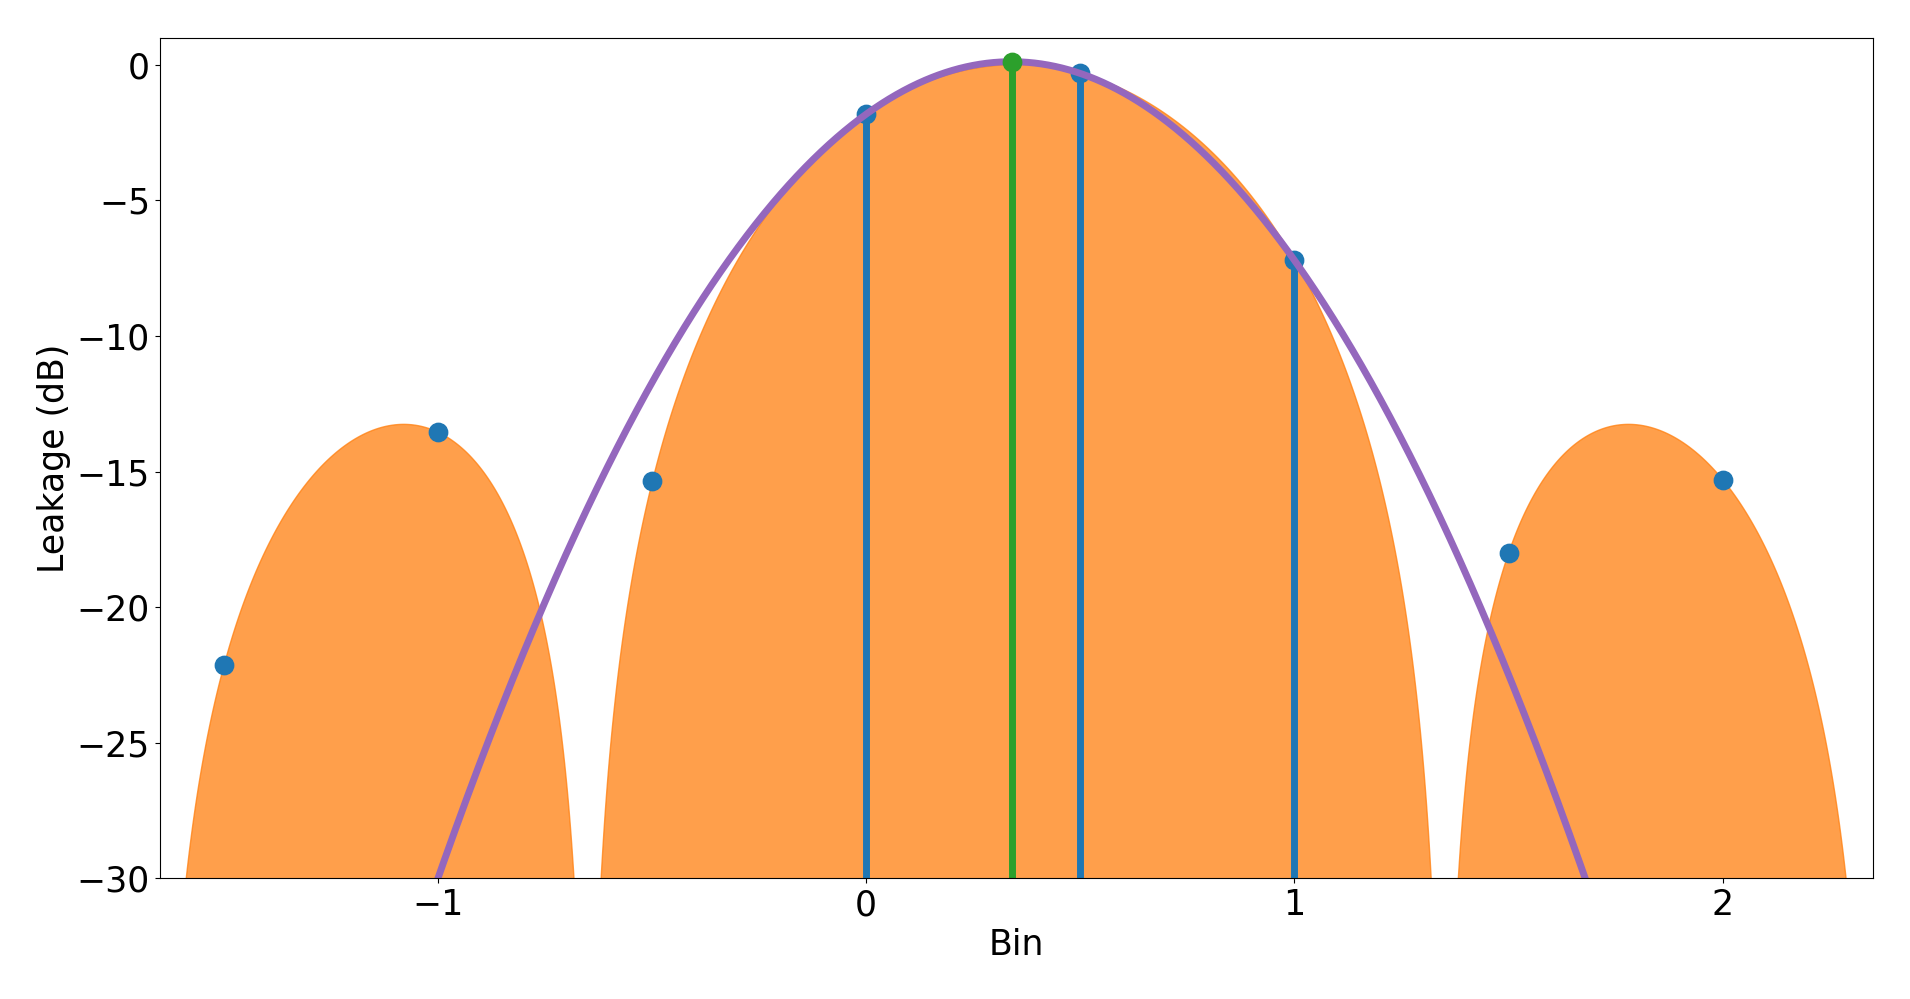
\includegraphics[width=0.90\linewidth]{figures/qifft.png}
    \end{figure}
\end{frame}
\logo{
\includegraphics[width=0.225\textwidth]{figures/logoleiden}}


% We are still left with two shortcomings of the basic estimator. These problems stem from the fact we simply pick the loudest bin as our estimation. If we instead first find all significant peaks, we can then carefully determine what note is played from the set of selected peaks.
\begin{frame}
\frametitle{HighRes estimator}
    {\large \textbf{Peak picking and note selection}}
    \bigskip

    Basic estimator shortcomings:
    \begin{itemize}
        \item No silence
        \item Octave problem
    \end{itemize}
    \bigskip

    {\LARGE \rotatebox[origin=c]{180}{$\Lsh$}} Solved by:
    % {\LARGE \rotatebox[origin=c]{180}{$\Lsh$}} Isolate peak picking and note selection
    \begin{itemize}
        \item Pick significant peaks
        \item Determine played note from picked peaks
    \end{itemize}
\end{frame}
% \begin{frame}
% \frametitle{HighRes estimator}
%     {\large \textbf{Peak picking and note selection}}
%     \begin{itemize}
%         \item Basic estimator shortcomings:
%         \begin{itemize}
%             \item No silence
%             \item Octave problem
%         \end{itemize}
%         \addtolength{\itemindent}{2mm}
%         \vspace*{-1.5mm}\item[{\LARGE \rotatebox[origin=c]{180}{$\Lsh$}}] Isolate peak picking and note selection
%     \end{itemize}
%     % {\large Basic estimator shortcomings}
%     % \begin{itemize}
%     %     \item No silence
%     %     \item Octave problem
%     % \end{itemize}
%     % \vspace*{-1.5mm}{\LARGE \rotatebox[origin=c]{180}{$\Lsh$}} Isolate peak picking and note selection
%     % \bigskip

%     % Peak pickers:
%     % \begin{itemize}
%     %     \item All local maxima %peaks ($b_{i-1} < b_i > b_{i+1}$)
%     %     \item Gaussian peak picking
%     % \end{itemize}
% \end{frame}


% Our pitch estimator relies on Gaussian peak picking. Here, we determine if a peak is significant using the Gaussian envelope of the spectrum. The Gaussian envelope is a moving average of the signal where the weights are determined by the Gaussian function as seen on the right. On the left, we can see a spectrum and its Gaussian envelope. Here, we can see the peaks from small noisy lobes from spectral leakage close to high peaks are filtered by the envelope.
\begin{frame}
\frametitle{HighRes estimator}
    \large{\textbf{Gaussian peak picking}}
    \begin{itemize}
        \item Gaussian envelope
        \item Moving average of spectrum
        \item Eliminates spectral leakage noise
    \end{itemize}
    \smallskip
    \smallskip

    \hspace{+3mm}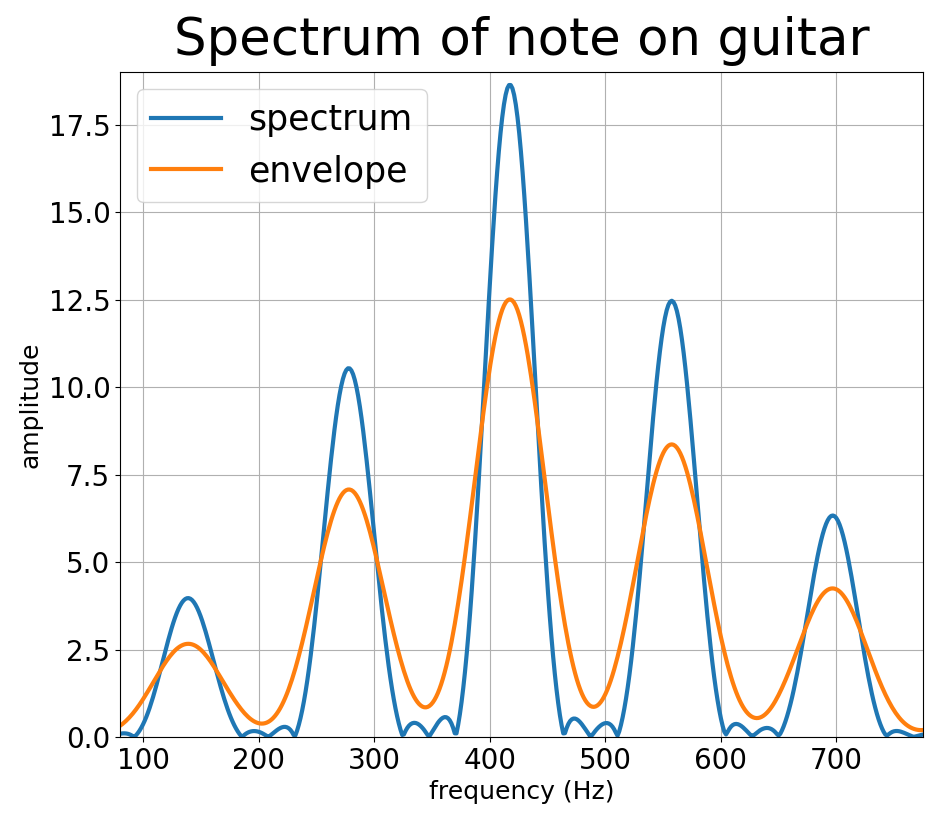
\includegraphics[width=0.47\linewidth]{figures/gaus_spec.png}

    \tikz[remember picture, overlay] {\node[right, anchor=east, outer sep=3.5mm] at (current page.east) {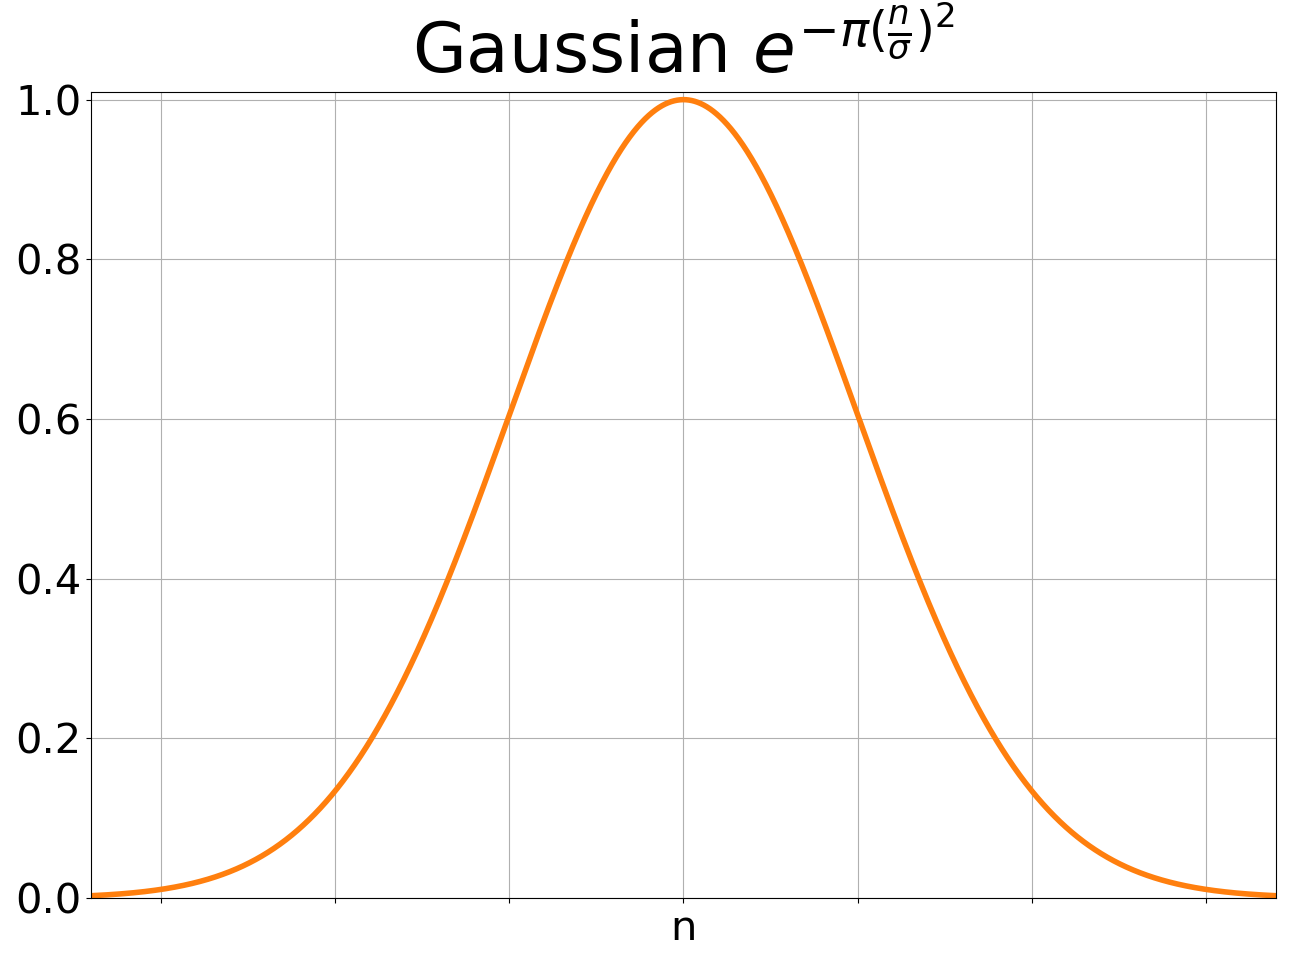
\includegraphics[width=0.43\linewidth]{figures/gaus.png}};}
\end{frame}


% Now we have obtained a set of significant peaks from our peak picker. Let us start by interpolating the actual peak locations using QIFFT. Our basic estimator would now simply pick the loudest peak. Instead, we can look for a group of peaks which form a valid series of overtones. Then, we select the peak with the most overtones as our estimate.
% We use multiple filters to further filter wrong estimations. Unfortunately, we do not seem to have enough time to go over them.
\begin{frame}
\frametitle{HighRes estimator}
    {\large \textbf{Note selection}}
    \begin{itemize}
        \item Set of peaks from peak picker
        \item QIFFT each peak
        \item Basic estimator: loudest peak
        \item Groups of overtones
        % \begin{itemize}
        %     \item Overtone error
        % \end{itemize}
    \end{itemize}
    \bigskip

    {\large \textbf{Filtering}}
    \begin{itemize}
        \item Minimum peak/envelope/signal power
        \item Instrument range filter
        \item Signal-to-noise filter
        % \item Transient filter
    \end{itemize}
\end{frame}


% If we put everything we've discussed together, we get our HighRes estimator. This estimator first...
\begin{frame}
\frametitle{HighRes estimator}
    \large{\textbf{HighRes estimator}}
    \begin{enumerate}
        \item Window function
        \item Fourier transform
        \item Calculate amplitudes
        \item Calculate Gaussian envelope
        \item Pick peaks
        \item Interpolate peaks
        \item Select note
    \end{enumerate}
    \smallskip
    
    Note that the input signal is overlapped and zero-padded
    \smallskip

    Additional filtering at every stage
\end{frame}


% In order work with our estimator, we created a program called Digistring. Digistring can feed arbitrary estimators samples from different sources. The estimator than creates note events, which represent the note estimations. Using these note events, we can generate graphics which may help funetuning estimators, synthesize sound and drive existing synthesizers or write the results to a file, allowing us to perform experiments on estimators. Instead of further discussing Digistring, I'll show it during a small demo at the end.
\begin{frame}
\frametitle{Digistring}
    \begin{figure}[H]
        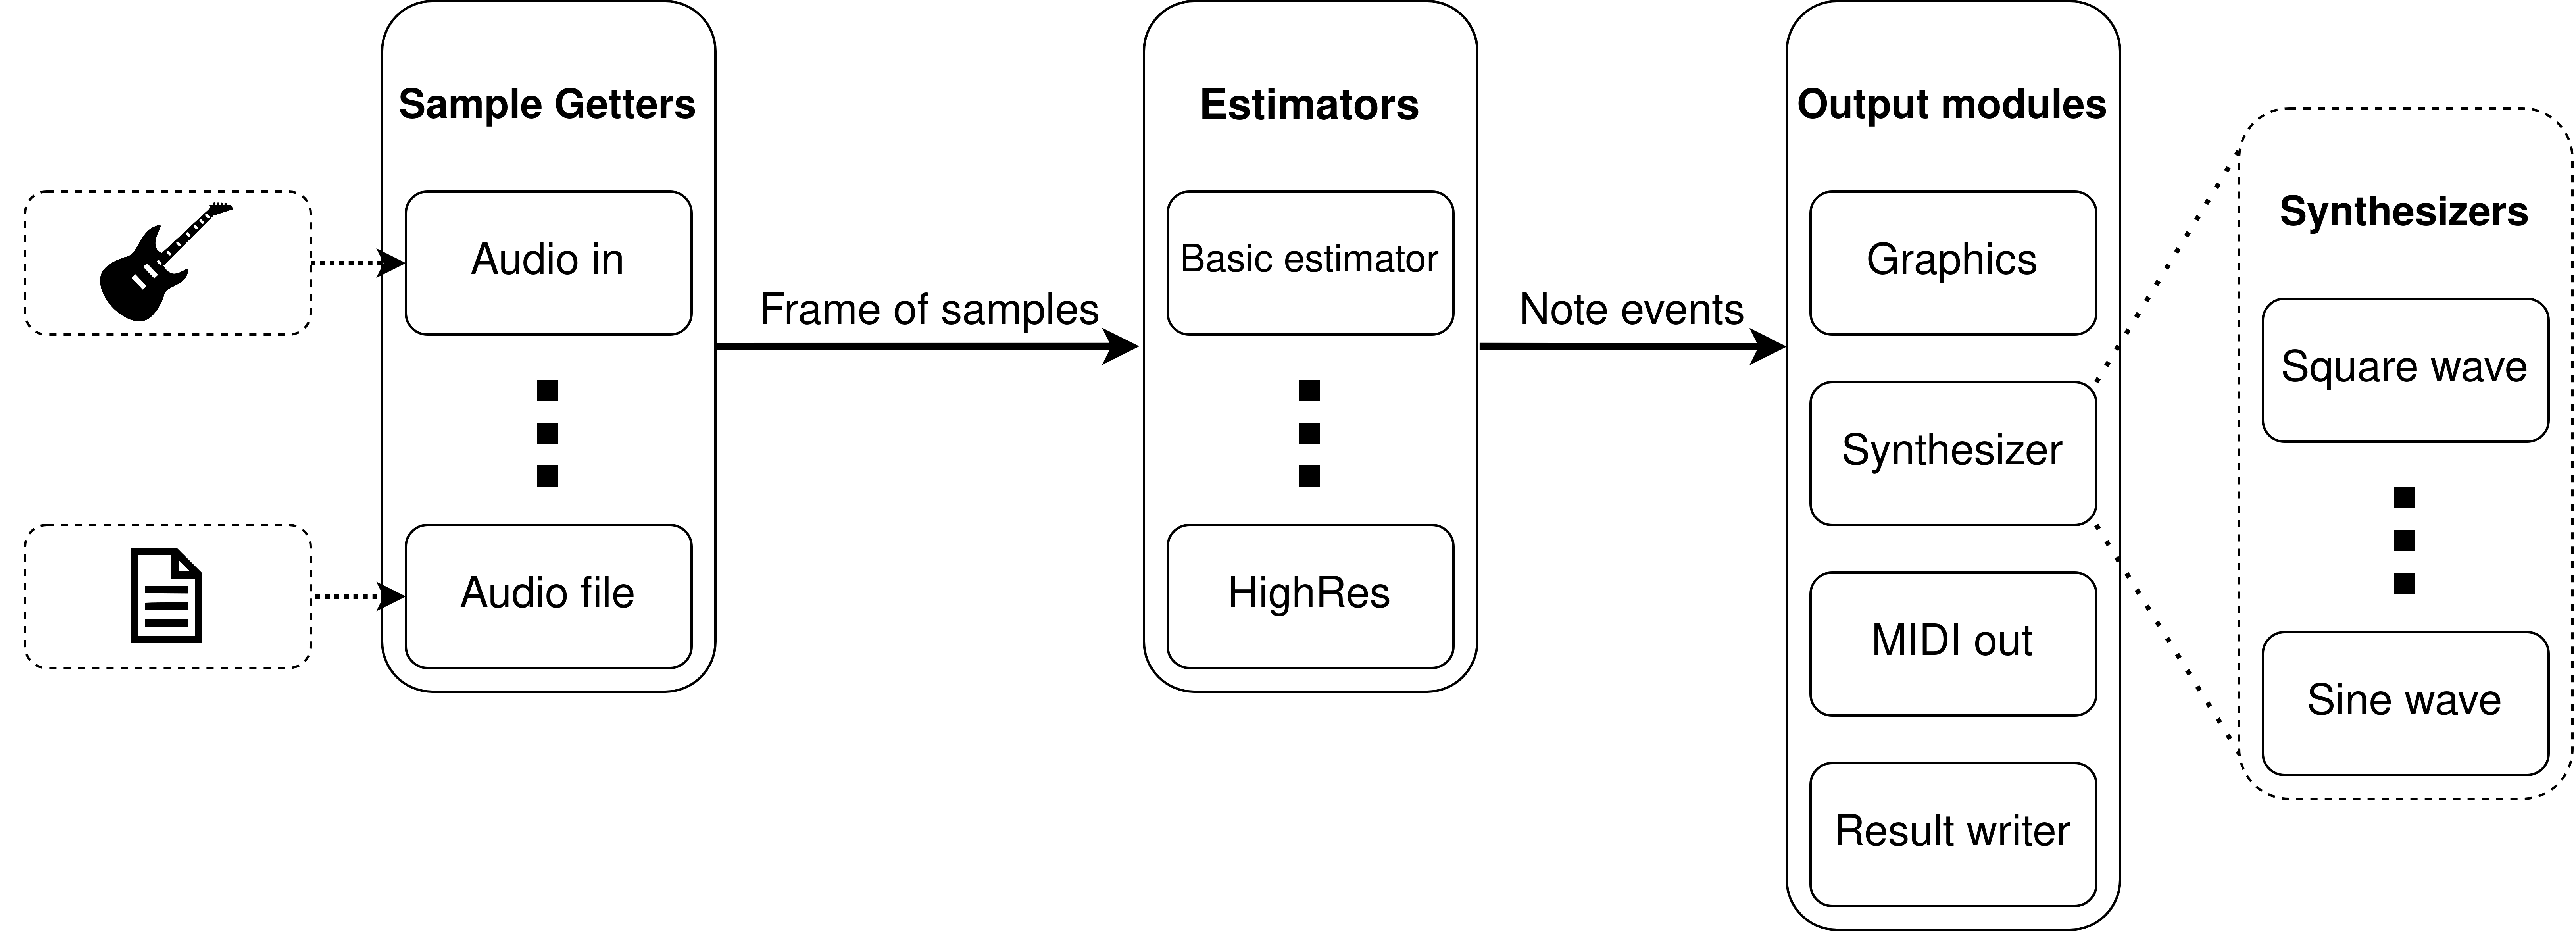
\includegraphics[width=0.90\linewidth]{figures/digistring_overview2.png}
    \end{figure}
\end{frame}


% % 
% \begin{frame}
% \frametitle{Experiments}
%     \centering{\Large \textbf{QIFFT errors} (Hz)}
%     \smallskip
%     \smallskip

%     \begin{tabular}{c|ccc}
%         Method & mean squared error & mean error & max error \\
%         \hline
%         Nearest bin                     & 0.179 & 0.366 & 0.732 \\
%         MQIFFT                          & 0.049 & 0.198 & 0.318 \\
%         LQIFFT with $\ln$               & 0.020 & 0.127 & 0.243 \\
%         LQIFFT with $\log_2$            & 0.020 & 0.127 & 0.243 \\
%         LQIFFT with $\log_{10}$         & 0.020 & 0.127 & 0.243 \\
%         dB-QIFFT ($20 * \log_{10}$)     & 0.020 & 0.127 & 0.243 \\
%         XQIFFT ($\epsilon = -0.301939$) & 0.017 & 0.114 & 0.416 \\
%         XQIFFT ($\epsilon = -0.764585$) & 0.023 & 0.107 & 0.604 \\
%         XQIFFT ($\epsilon = 0.0554724$) & 0.021 & 0.130 & 0.213
%     \end{tabular}
%     \bigskip

%     bin size $\approx$ 1.465 Hz
% \end{frame}
% \begin{frame}[noframenumbering]
% \frametitle{Experiments}
%     \centering{\Large \textbf{QIFFT errors} (Hz)}
%     \smallskip
%     \smallskip

%     \begin{tabular}{c|ccc}
%         Method & mean squared error & mean error & max error \\
%         \hline
%         Nearest bin                     & 0.179 & 0.366 & 0.732 \\
%         MQIFFT                          & 0.049 & 0.198 & 0.318 \\
%         \rowcolor{yellow}LQIFFT with $\ln$               & 0.020 & 0.127 & 0.243 \\
%         \rowcolor{yellow}LQIFFT with $\log_2$            & 0.020 & 0.127 & 0.243 \\
%         \rowcolor{yellow}LQIFFT with $\log_{10}$         & 0.020 & 0.127 & 0.243 \\
%         \rowcolor{yellow}dB-QIFFT ($20 * \log_{10}$)     & 0.020 & 0.127 & 0.243 \\
%         XQIFFT ($\epsilon = -0.301939$) & 0.017 & 0.114 & 0.416 \\
%         XQIFFT ($\epsilon = -0.764585$) & 0.023 & 0.107 & 0.604 \\
%         XQIFFT ($\epsilon = 0.0554724$) & 0.021 & 0.130 & 0.213
%     \end{tabular}
%     \bigskip

%     bin size $\approx$ 1.465 Hz
% \end{frame}
% \begin{frame}[noframenumbering]
% \frametitle{Experiments}
%     \centering{\Large \textbf{QIFFT errors} (Hz)}
%     \smallskip
%     \smallskip

%     \begin{tabular}{c|ccc}
%         Method & mean squared error & mean error & max error \\
%         \hline
%         Nearest bin                     & 0.179 & 0.366 & 0.732 \\
%         MQIFFT                          & 0.049 & 0.198 & 0.318 \\
%         LQIFFT                          & 0.020 & 0.127 & 0.243 \\
%         XQIFFT ($\epsilon = -0.301939$) & 0.017 & 0.114 & 0.416 \\
%         XQIFFT ($\epsilon = -0.764585$) & 0.023 & 0.107 & 0.604 \\
%         XQIFFT ($\epsilon = 0.0554724$) & 0.021 & 0.130 & 0.213
%     \end{tabular}
%     \bigskip

%     bin size $\approx$ 1.465 Hz
% \end{frame}


% In order to determine the performance of Digistring, we ran a few experiments.
% First, we set out to determine the minimum frame length we can get away with. As mentioned earlier, we want small frame lengths to minimize latency. Our limiting factor is the minimum Fourier resolution to discern the two lowest notes on a guitar.
% For our first experiment, we looked at the minimum frame length to discern two pure sine waves. This serves as a theoretical lower bound on frame length. We found we need a frame time of about 5 milliseconds.
% When using actual recordings of the notes played on a guitar, we needed at least 30 milliseconds to reliably discern the two notes. However, due to the low Fourier resolution, the note estimates are dissonant. We found we need a frame length of about 43 milliseconds to get consonant note estimations.
\begin{frame}
\frametitle{Experiments}
    {\large \textbf{Fourier size limit}}
    \begin{itemize}
        \item Resolution vs latency
        \item Lowest notes (\notee{E}{2} and \notee{F}{2})
        \item Pure sines: 5.33 ms
        \item Recordings: 30 ms
        \begin{itemize}
            \item[{\LARGE \rotatebox[origin=c]{180}{$\Lsh$}}] Dissonant
        \end{itemize}
        \item Digistring: 42.67 ms
    \end{itemize}
\end{frame}


% Next up, we measured the speed of pitch estimation. The total latency of Digistring is the frame length plus the processing time. In this image, we can see the total processing time of a frame is about 1 millisecond. This is negligable compared to the frame length. Most time is spend on performing the Fourier transform.
\logo{}
\begin{frame}
\frametitle{Experiments}
    \centering{\Large \textbf{Pitch estimation speed}}
    \begin{figure}[H]
        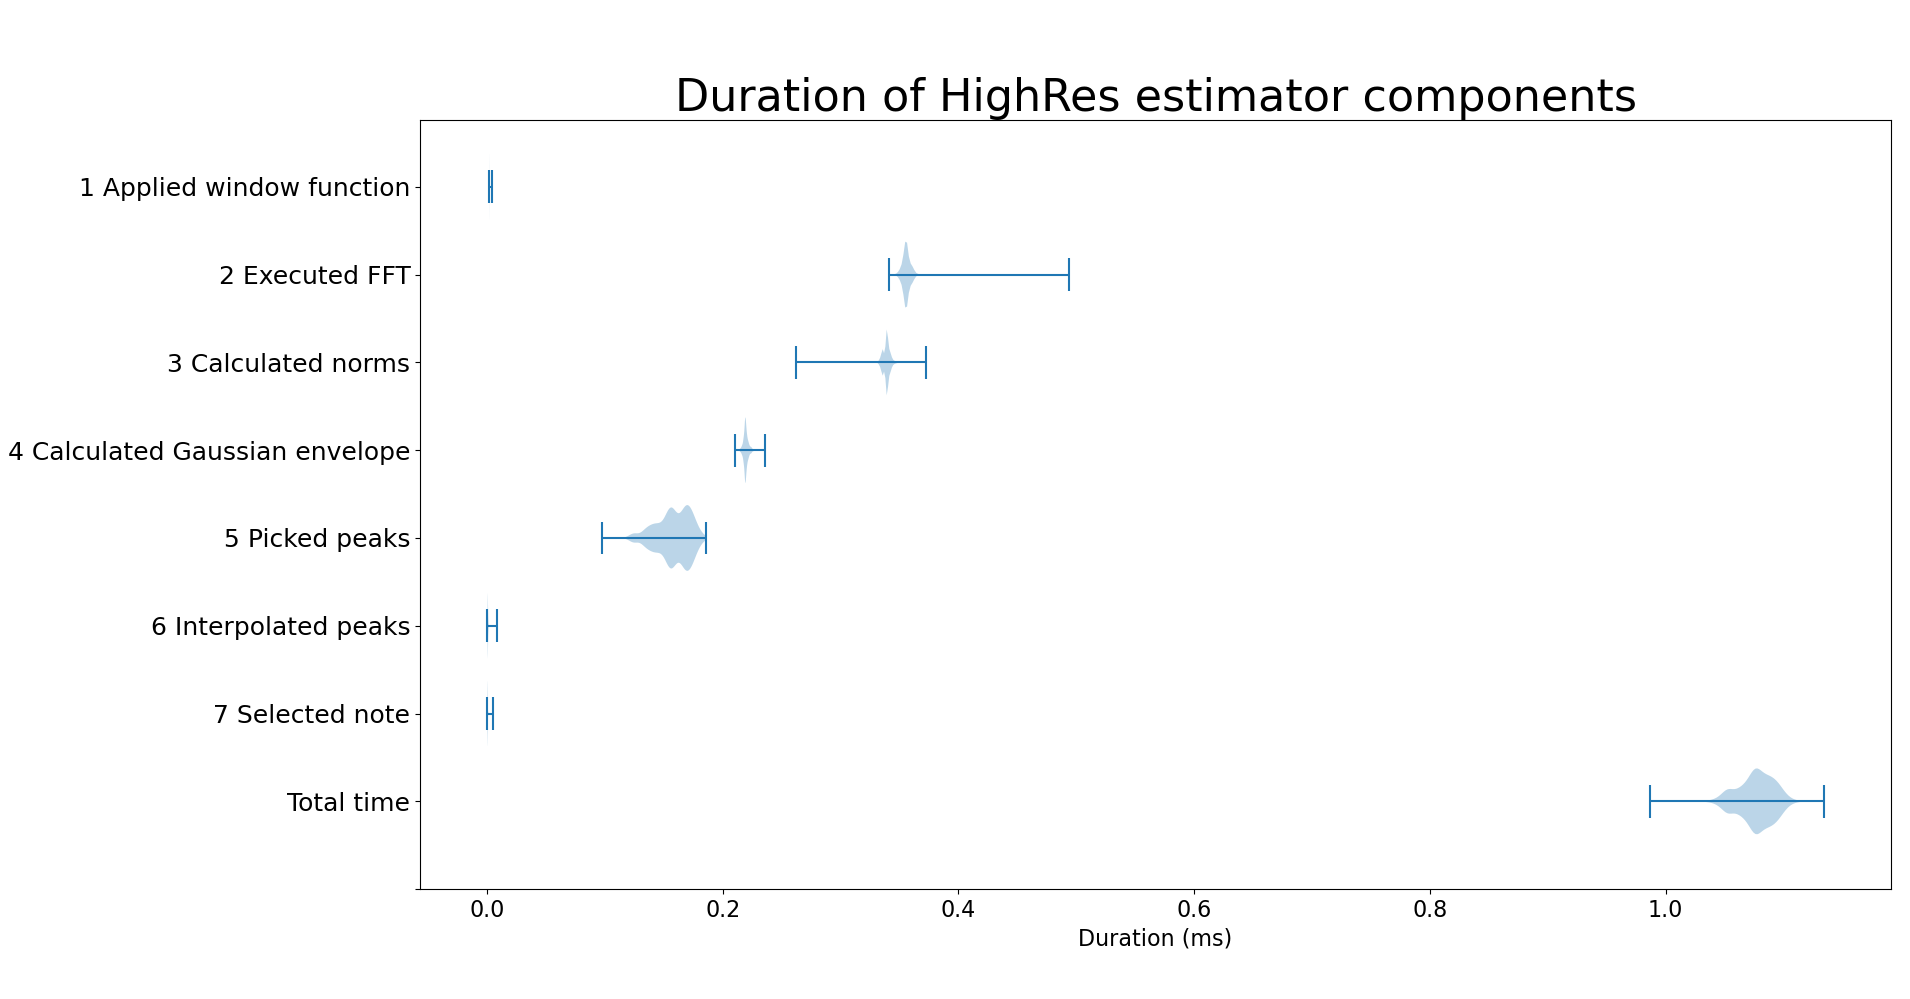
\includegraphics[width=\linewidth]{figures/perfplot.png}
    \end{figure}
\end{frame}
\logo{
\includegraphics[width=0.225\textwidth]{figures/logoleiden}}


% % 
% \begin{frame}
% \frametitle{Experiments}
%     {\large \textbf{Performance discussion}}
%     \begin{itemize}
%         \item Playing guitar $\not =$ playing guitar synth
%         \item Play clean/careful
%         \item Monophonic $\rightarrow$ unused string muting
%         \item Palm muting
%         \item Hammer-on/pull-off and tapping
%         \item Don't double pick/shred
%         \item Bending
%         \item Latency
%     \end{itemize}
% \end{frame}


% To determine the accuracy of our pitch estimation, we ran the Fraunhofer dataset through Digistring. The Fraunhofer dataset constains both monophonic and polyphonic recordings. As we perform monophonic transcription, we only use the monophonic subset. The dataset consists of three monophonic subsets. Unfortunately, obtaining well annotated datasets is a big problem in pitch estimation research. Consequently, the dataset is not wel suited for our needs, however, it'll have to do.
\begin{frame}
\frametitle{Experiments}
    {\large \textbf{Pitch estimation accuracy}}
    \begin{itemize}
        \item Fraunhofer dataset
        \item Polyphonic $\rightarrow$ use a subset
        \item 4 subsets, 3 monophonic
        \item Challenging dataset
    \end{itemize}
\end{frame}


% The first subset contains single note recording of all positions up to the 12th fret for every string. All these positions are recorded on two guiters, and on one of the guitars different pick-up configurations were used.
% In the table, we can see we did correctly identify every note. Most of the time, we found more than 90% of the note correctly. In the last column, we see that the estimated note event often doesn't consist of one long event, but has some interruption.
% In the table, we can see significantly different results bewteen the different guitars and pick-up configurations. We were not able to reproduce these results with any of our guitars, every guitar and pick-up configuration performs about the same. The differences are likely due to inconsistent playing quality in the dataset.
\begin{frame}
\frametitle{Experiments}
    {\large \textbf{First subset}}
    \begin{itemize}
        \item Single note recordings
        \item All positions up to $12^{\text{th}}$ fret
        \item Every string
        \item 2 guitars
        \item 3 different pick-up combinations
    \end{itemize}
    \bigskip

    \hspace{+8mm}\begin{tabular}{r|rrr}
        version     & correct & $t_{>0.9}$ correct & no interrupt \\
        \hline
        Fender      & 100 \%  & 96 \%   & 81 \% \\
        Ibanez N    & 100 \%  & 96 \%   & 76 \% \\
        Ibanez B    & 100 \%  & 87 \%   & 51 \% \\
        Ibanez N+B  & 100 \%  & 92 \%   & 67 \%

    \end{tabular}
\end{frame}


% The second subset consists of 6 guitar licks played on three different guitar. All licks are played with plectrum and with finger style.
% Again, we correctly identify every note, however, often we only find around 80% of the note. There is a large difference between finger style playing and playing with a pick. When playing finger style, the transients are significantly softer, however, the sustaining signal is often much noisier.
\begin{frame}
\frametitle{Experiments}
    {\large \textbf{Second subset}}
    \begin{itemize}
        \item 6 guitar licks
        \item 3 guitars
        \item Plectrum and finger style
    \end{itemize}
    \bigskip

    \hspace{+8mm}\begin{tabular}{r|rr}
        version          & correct & $t_{>0.8}$ correct \\
        \hline
        Fender pick      & 100 \%  & 83 \% \\
        Fender finger    & 100 \%  & 58 \% \\
        Gibson pick      & 100 \%  & 75 \% \\
        Gibson finger    & 100 \%  & 58 \% \\
        Aristides pick   & 100 \%  & 79 \% \\
        Aristides finger & 100 \%  & 63 \%
        % total            & 100 \%  & 69 \%
    \end{tabular}
\end{frame}


% The last subset consists of two excerpts of classical pieces. Instead of going over the numbers again, I'll show you the estimations visualized. The annotations are shown in orange and the green and red lines show the correct and incorrect estimated note events. We can see that we generally estimate the correct note for most of the duration of a note. In these two pieces, all errors were either at the onset or offset of a note, likely from transients. This second image is very similar, only errors at onsets or offsets. Here we can see a small error, however, this is an error in the dataset, as it is supposed to be monophonic but there are two orange lines at one timepoint.
\begin{frame}
\frametitle{Experiments}
    {\large \textbf{Third subset}}
    \begin{itemize}
        \item 5 excerpts of classical pieces
        \begin{itemize}
            \item[{\LARGE \rotatebox[origin=c]{180}{$\Lsh$}}] Only 2 monophonic
        \end{itemize}
    \end{itemize}

    \begin{figure}[H]
        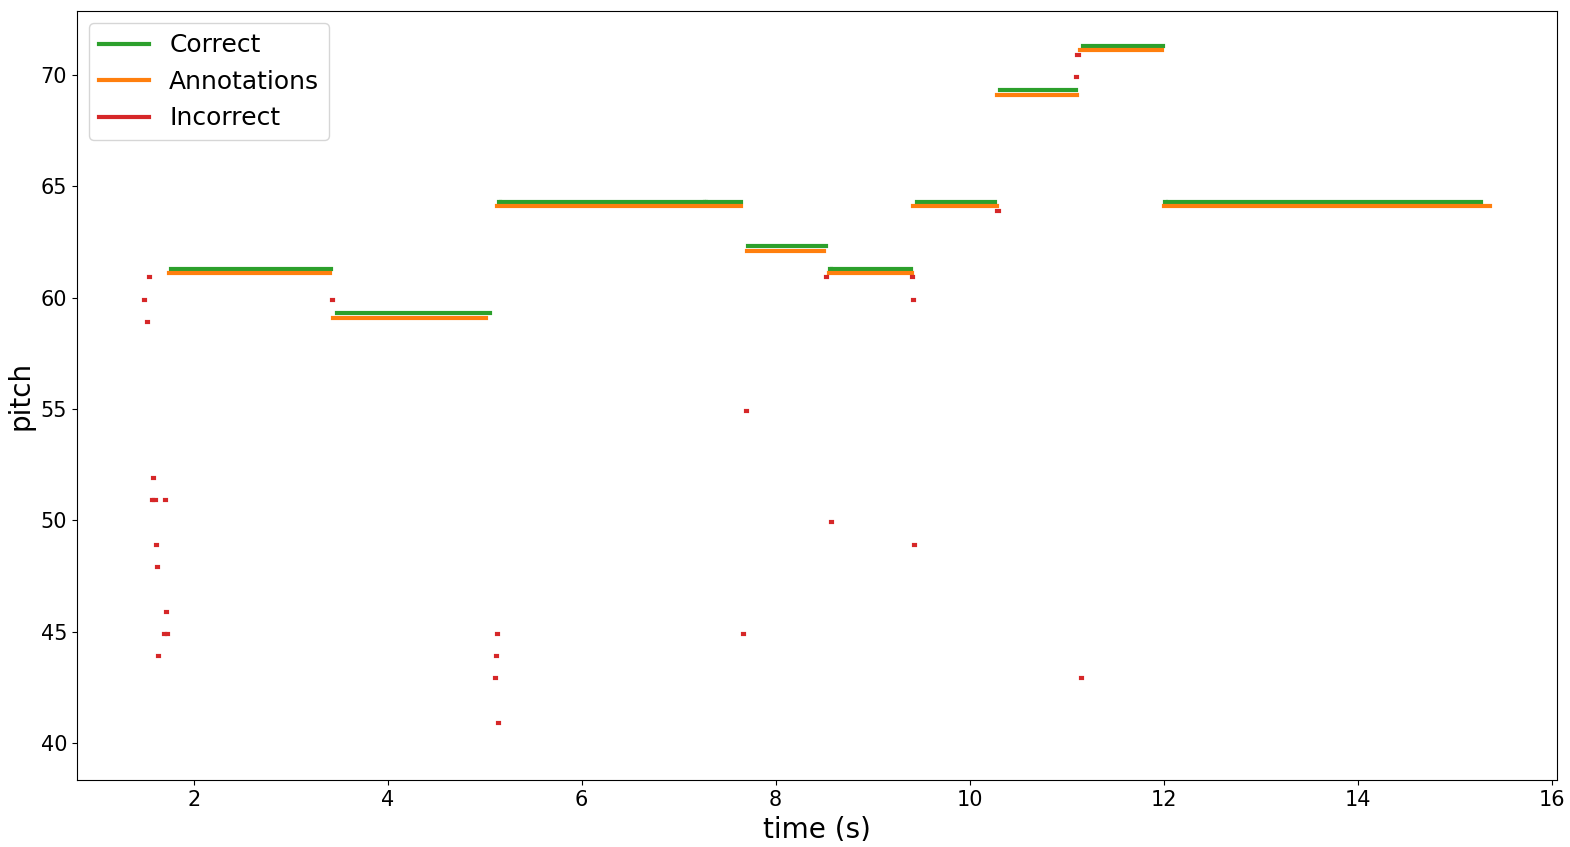
\includegraphics[width=\linewidth]{figures/dataset3-1.png}
    \end{figure}
\end{frame}
\logo{}
\begin{frame}
\frametitle{Experiments}
    \begin{figure}[H]
        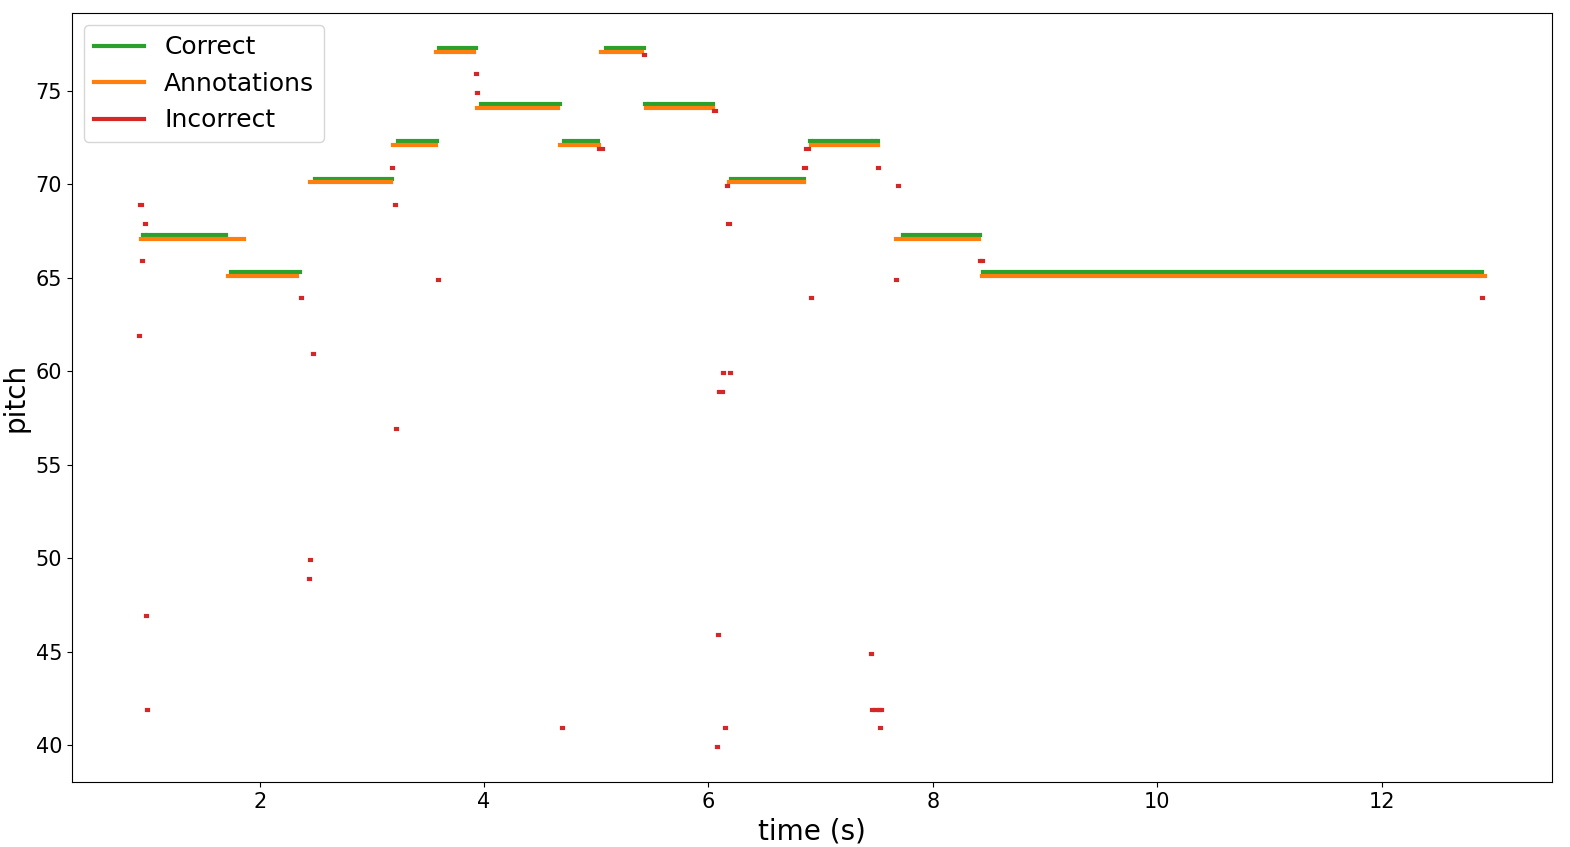
\includegraphics[width=\linewidth]{figures/dataset3-2.png}
    \end{figure}
\end{frame}
\logo{
\includegraphics[width=0.225\textwidth]{figures/logoleiden}}


% So let me summerize what I've done. In this thesis, I constructed a Fourier transform based real-time pitch estimation algorithm, accompanied by a framework which can host this algorithm and synthesize sound based on the estimation. It also provides tools to perform experiments on pitch estimators.
% During our research, we found that we are limited by the amount of frequency resolution on low frame lengths, which we need to minimize the latency. We managed to push the latency from 200 milliseconds down to 43 milliseconds through interpolation. This is however not enough to meet our real-time constraint. Note however that our frame length is limited by the lowest two notes we want to discern, so we could easily make our real-time constraint by choosing a higher lowest note.
\begin{frame}
\frametitle{Conclusions}
    {\large \textbf{Contributions}}
    \begin{itemize}
        \item HighRes estimator
        \item Digistring
    \end{itemize}
    \bigskip

    {\large \textbf{Conclusions}}
    \begin{itemize}
        \item Limited by Fourier resolution $\Leftrightarrow$ latency
        \item 200 ms frame $\rightarrow$ 43 ms frame
        \item Real-time constraint $\Leftrightarrow$ lowest note
    \end{itemize}
\end{frame}


% And now for the most important part, the demo. No matter how many experiments we perform, in the end, the only important performance factor is if the estimator is musically sound.
% ...\
%Playing guitar $\not =$ playing guitar synth (rake bij windowpane, end of mother solo)
%Play clean/careful (green tinted sixties minds)
%Monophonic $\rightarrow$ unused string muting (clairvoyant)
%Palm muting (necrophantasia pianoteq)
%However, palm muting doesn't fix everything (coldshot, John Pertrucci)
%Hammer-on/pull-off and tapping (the metal, god blessed video, bach tap)
%Don't double pick/shred (thrive, miserloe, gojira)
%Bending (cause we ended as lovers)
%Latency ()
\begin{frame}
\frametitle{Digistring demo}
    \begin{center}
        {\huge \textbf{Digistring demo}}
    \end{center}
\end{frame}


\end{document}
